\section*{Цель}

Исследование характеристик процесса рождения и гибели.

\section*{Порядок выполнения}

\begin{enumerate}
    \item Разработать программу для моделирования процесса рождения и гибели.
    На экран выводить диаграмму состояний процесса и графики значений вероятностей попадания в первые одиннадцать состояний из нулевого состояния, математического ожидания и дисперсии процесса.
    \item Исследовать поведение процесса при заданных последовательностях параметров { $\lambda_k$ }, { $\mu_k$ } при различных начальных условиях.
    \item Охарактеризовать поведение процесса при заданных последовательностях параметров { $\lambda_k$ }, { $\mu_k$ }.
\end{enumerate}

\section*{Исходные данные}

Задана последовательности параметров \{ $\lambda_k$ \} и \{ $\mu_k$ \}, соответствующие трем моделям процесса рождения и
гибели.

\begin{align*}
    \lambda_k & = 0.4 & \mu_k & = 0.3\\
    \lambda_k & = 1.15k^3 + 1 & \mu_k & = 0.33k^3\\
    \lambda_k & = 0.7 / (k + 12)^2 & \mu_k & = 0.3 / k^2
\end{align*}

\section*{Диаграммы состояний}

Для каждой из моделей были построены диаграммы состояний процесса для предварительных прогонов каждой из моделей.

\begin{figure}[h!]
    \centering
    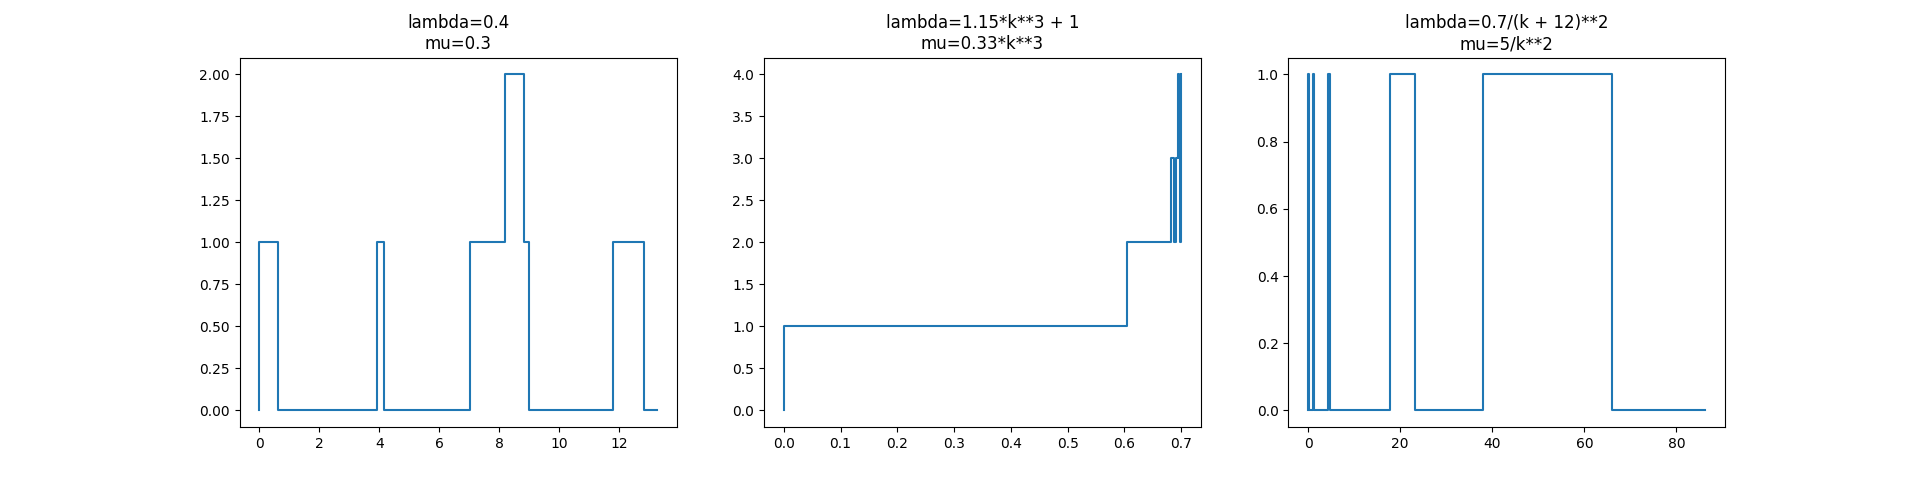
\includegraphics[width=\textwidth]{\jobname/docs/img/state_diagrams.png}
    \caption{Диграммы состояний процесса предварительных прогонов каждой модели}
\end{figure}

\section*{Первая модель, $\lambda_k = 0.4, \mu_k = 0.3$}

В качестве исследования заданной модели были произведены 200 экспериментов с целью определения вероятностей каждого
из состояний в каждый момент времени $P(X(t)=n)$, а также значений математического ожидания $M(X)$ и дисперсии $D(X)$.
Финальные вероятности для текущей модели не существуют, поскольку ряд $\sum_{k=1}^{\infty}\pi_k$ расходится.
Полученные графики вероятностей, математического ожидания и дисперсии приведены на графиках ниже.

\begin{figure}[h!]
    \centering
    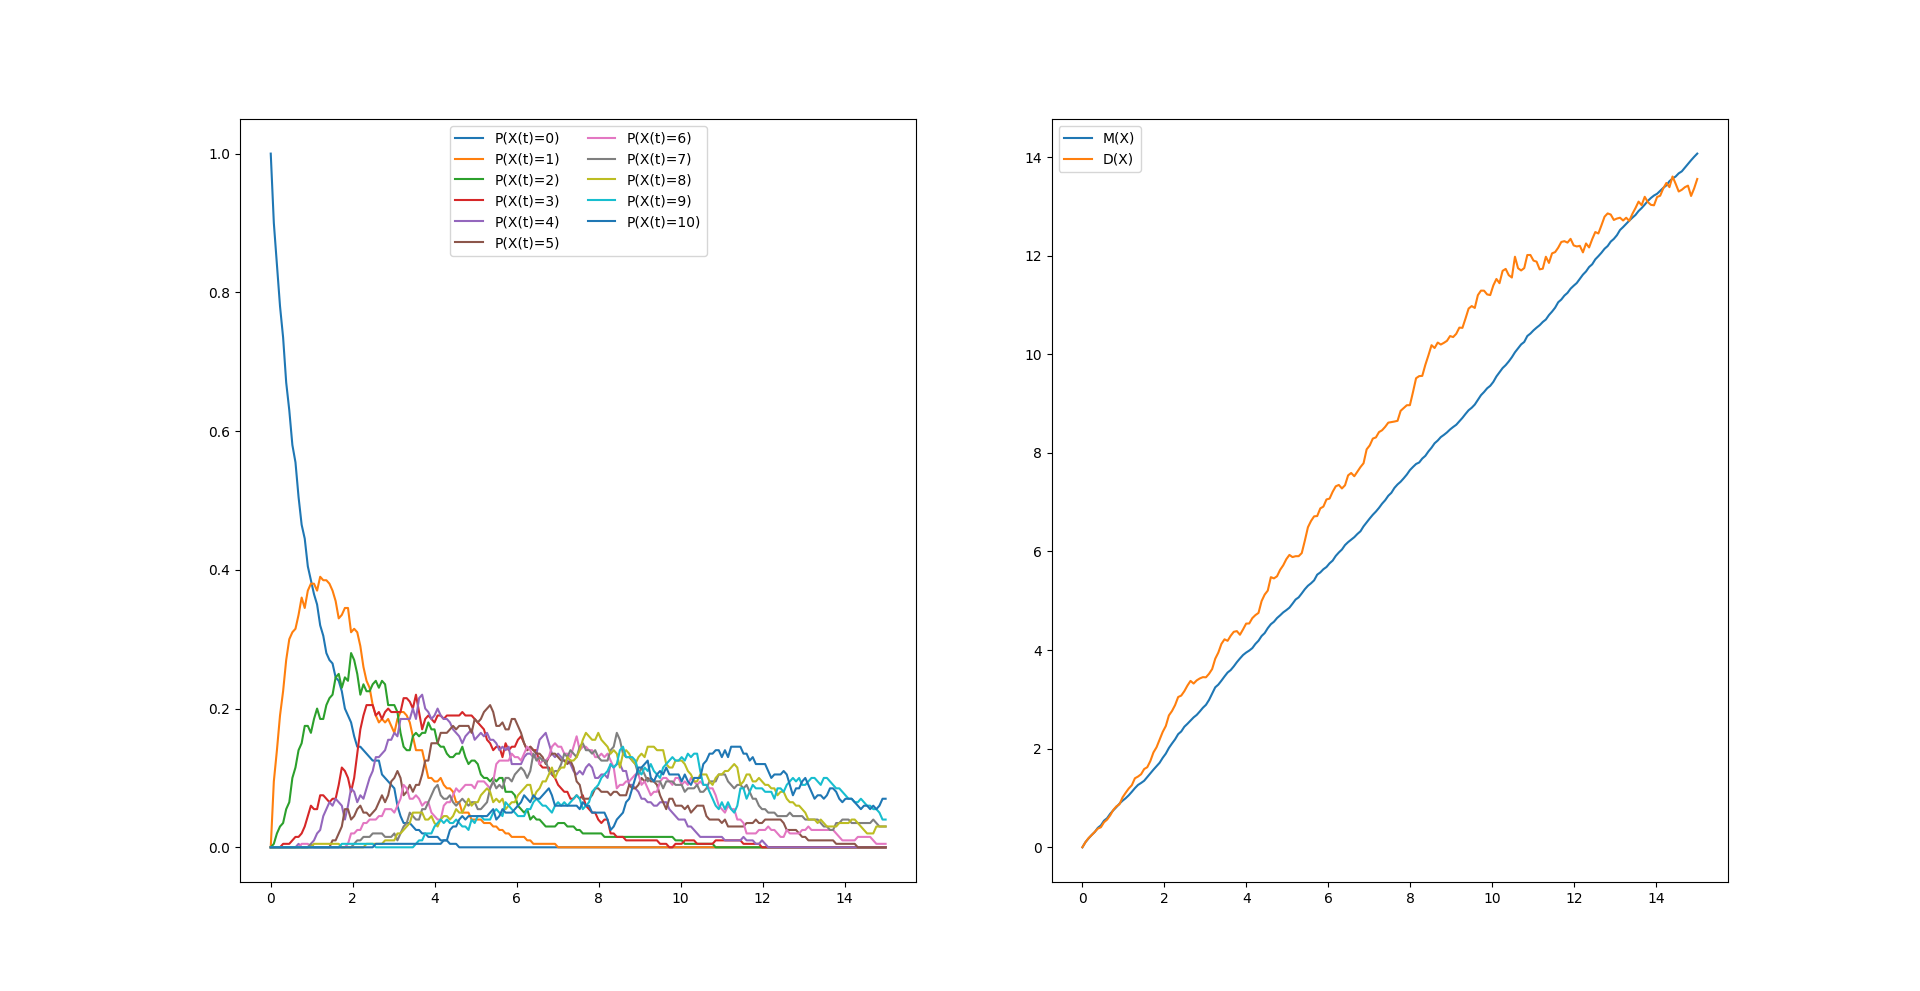
\includegraphics[width=\textwidth]{\jobname/docs/img/model_1.png}
    \caption{Графики вероятностей состояний, математического ожидания и дисперсии при $\lambda_k = 0.4, \mu_k = 0.3$}
\end{figure}

\newpage

\section*{Вторая модель, $\lambda_k = 1.15k^3 + 1, \mu_k = 0.33k^3$}

В качестве исследования заданной модели были произведены 200 экспериментов с целью определения вероятностей каждого
из состояний в каждый момент времени $P(X(t)=n)$, а также значений математического ожидания $M(X)$ и дисперсии $D(X)$.
Финальные вероятности для текущей модели не существуют, поскольку ряд $\sum_{k=1}^{\infty}\pi_k$ расходится.
Полученные графики вероятностей, математического ожидания и дисперсии приведены на графиках ниже.

\begin{figure}[h!]
    \centering
    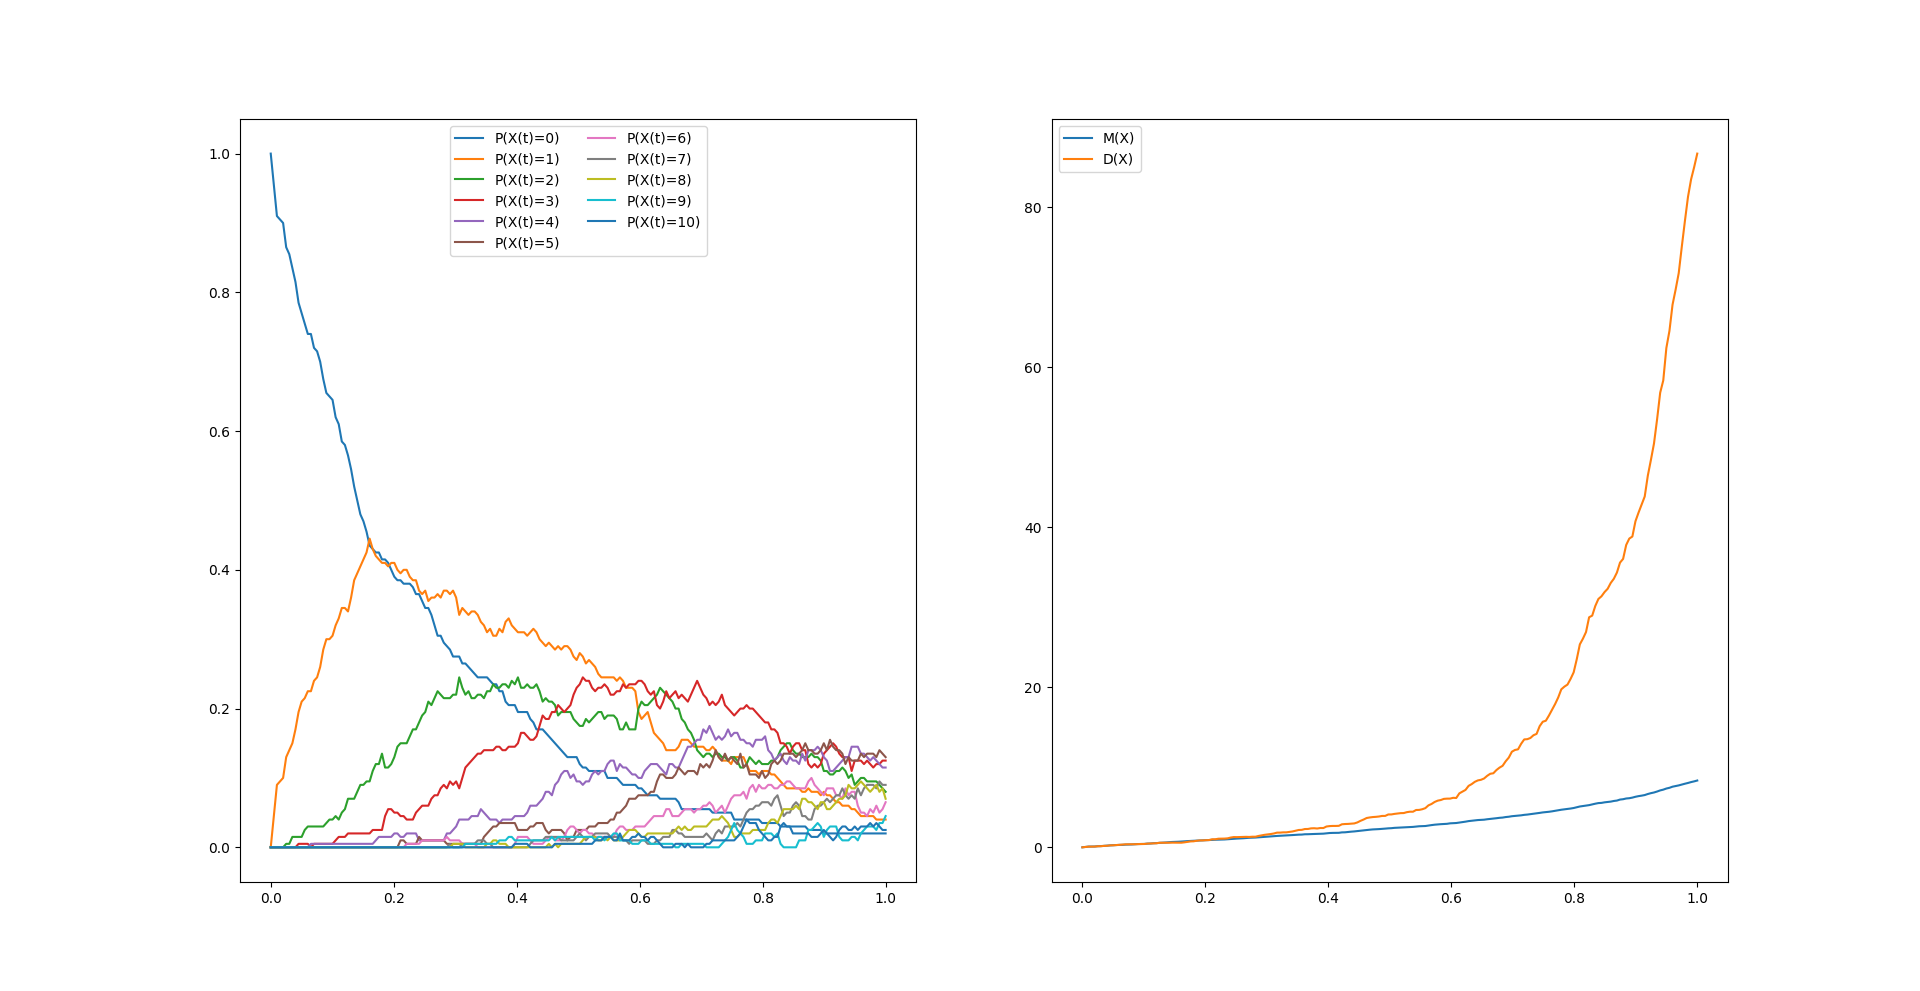
\includegraphics[width=\textwidth]{\jobname/docs/img/model_2.png}
    \caption{Графики вероятностей состояний, математического ожидания и дисперсии при $\lambda_k = 1.15k^3 + 1, \mu_k = 0.33k^3$}
\end{figure}

\newpage

\section*{Третья модель, $\lambda_k = 0.7 / (k + 12)^2, \mu_k = 0.3 / k^2$}

В качестве исследования заданной модели были произведены 200 экспериментов с целью определения вероятностей каждого
из состояний в каждый момент времени $P(X(t)=n)$, а также значений математического ожидания $M(X)$ и дисперсии $D(X)$.
Для настоящей модели ряд $\sum_{k=1}^{\infty}\pi_k$ сходится, поэтому финальные вероятности существуют и равны
для первого и второго состояния 0.5, а для всех остальных - нулю.

Полученные графики вероятностей, математического ожидания и дисперсии приведены на графиках ниже.

\begin{figure}[h!]
    \centering
    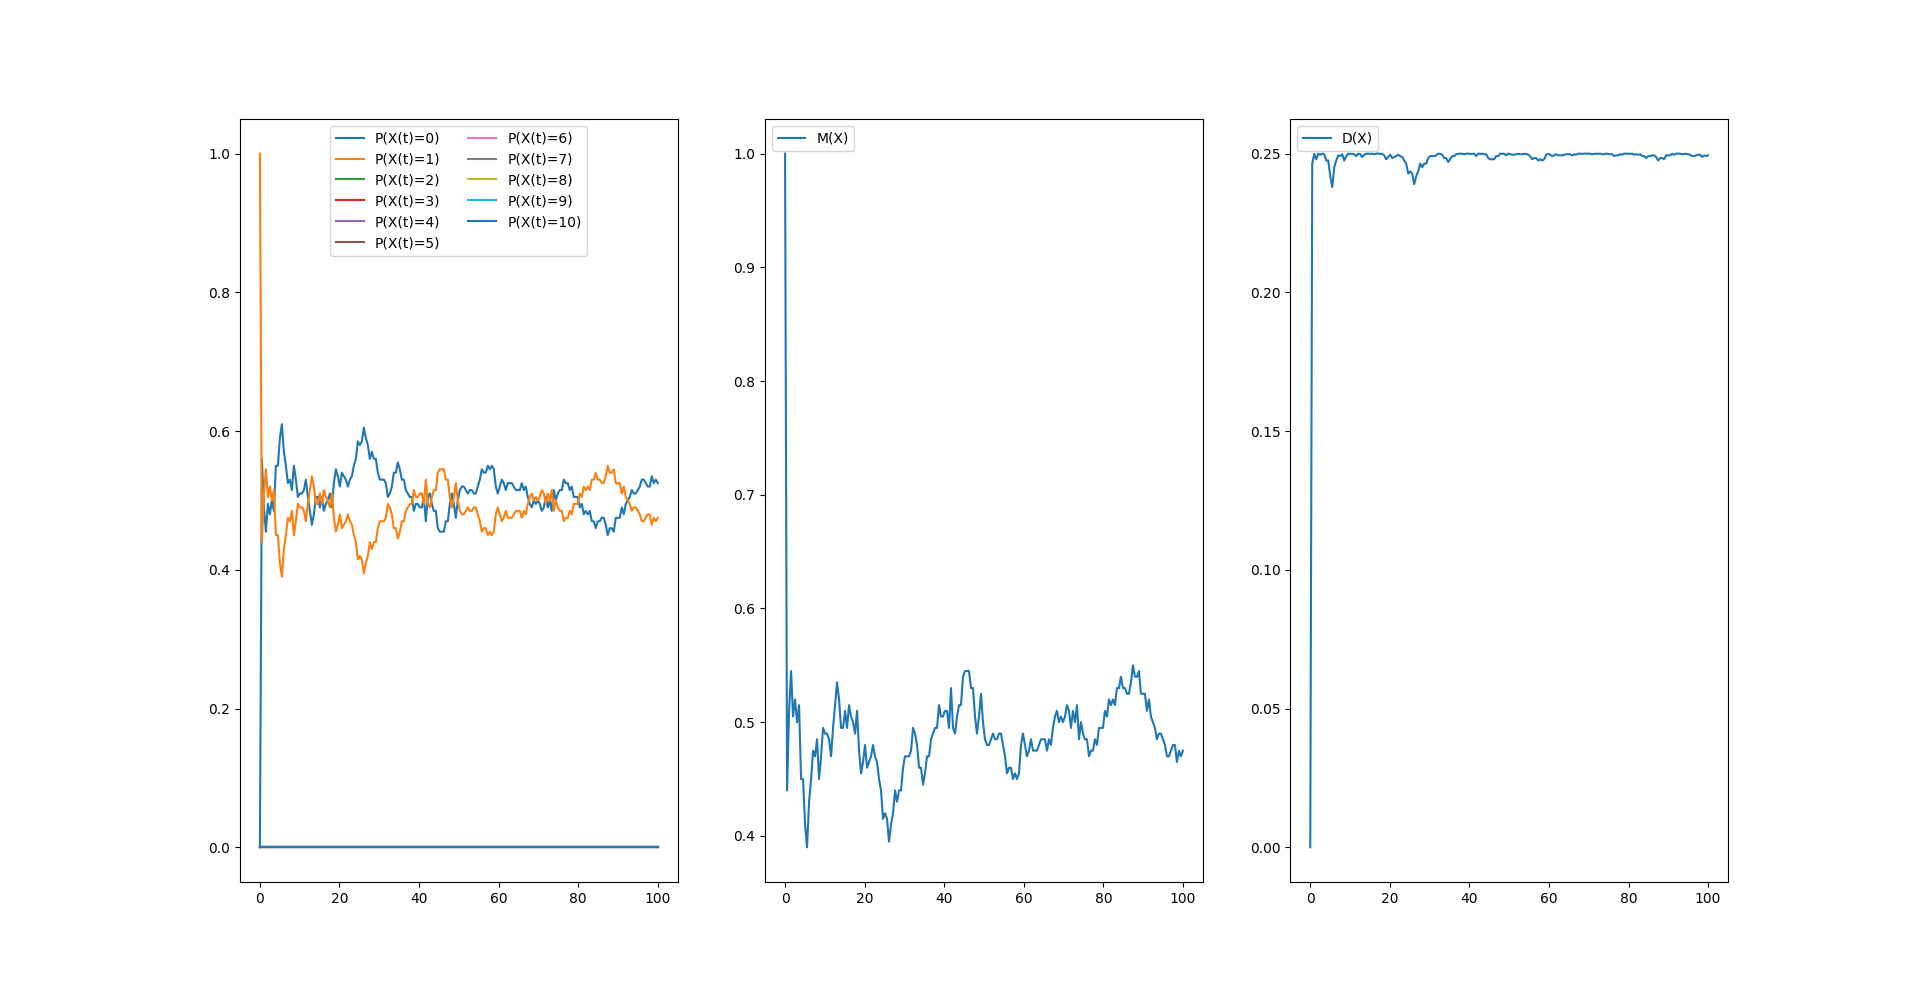
\includegraphics[width=\textwidth]{\jobname/docs/img/model_3.png}
    \caption{Графики вероятностей состояний, математического ожидания и дисперсии при $\lambda_k = 0.7 / (k + 12)^2, \mu_k = 0.3 / k^2$}
\end{figure}

\section*{Выводы}

В ходе выполнения лабораторной работы были исследованы три процесса рождения и гибели, заданные последовательностями
параметров \{ $\lambda_k$ \} и \{ $\mu_k$ \}.
Для каждой из моделей были построены диаграммы состояний, графики вероятности случайной величины, математического
ожидания и дисперсии в каждый момент времени.
На основе параметров моделей были составлены характеристики каждого из процессов, описанные ниже.

\subsection*{Первая модель}

В связи с независимостью $\lambda_n$ и $\mu_n$ от текущего состояния, общая интенсивность изменения числа особей с течением
времени $\lambda_n/\mu_n$ не меняется.
Можно наблюдать, что математическое ожидание и дисперсия растут практически линейно, что объясняется предыдущим
утверждением о постоянстве интенсивности изменения числа особей.

\subsection*{Вторая модель}

Во втором случае $\lambda_n$ и $\mu_n$ зависят от куба текущего состояния, что обеспечивает уменьшение времени
между событиями рождения и гибели с течением времени.
Кроме того интенсивность рождения растет быстет быстрее, чем интенсивность гибели.
Можно наблюдать, что скорости роста математического ожидания и дисперсии со временем увеличиваются, что согласуется с
предыдущим утверждением об уменьшении времени поступления новых событий.

\subsection*{Третья модель}

В последней модели $\lambda_n$ обратно зависит от значения текущего состояния, что обеспечивает увеличение времени поступления
заявок с течением времени.
Можно наблюдать, что спустя некоторое время математическое ожидание стабилизируется в районе 0.5, а дисперсия в районе
0.25, что согласуюется с расчитанными финальными вероятностями, которые равны состовляют 0.5 для первых двух состояний -
нуля и единицы.

\section*{Листинги}

\subsection*{Листинг основного скрипта}
\lstinputlisting[language=Python,texcl=true]{\jobname/lab.py}

\subsection*{Листинг скрипта, содержащего модель чистого рождения}
\lstinputlisting[language=Python,texcl=true]{\jobname/birth_death.py}

\subsection*{Листинг скрипта, содержащего генераторы}
\lstinputlisting[language=Python,texcl=true]{\jobname/../common/gen.py}

\subsection*{Листинг скрипта, содержащего утилиты}
\lstinputlisting[language=Python,texcl=true]{\jobname/../common/utils.py}

\subsection*{Листинг скрипта, инициализируещего логирование}
\lstinputlisting[language=Python,texcl=true]{\jobname/../common/log.py}
